\documentclass[tikz,border=3mm]{standalone}

\definecolor{fvmadaptedge}{HTML}{8A7E7E}
\definecolor{splitred}{HTML}{AF2525}

\begin{document}
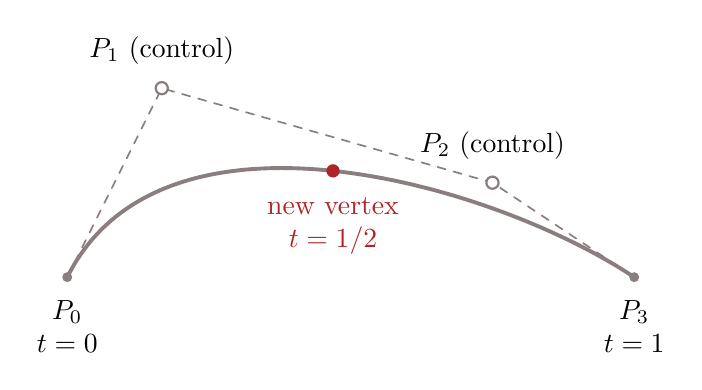
\begin{tikzpicture}[x=1.2cm,y=1.2cm,line cap=round,line join=round]
  \coordinate (P0) at (0,0);
  \coordinate (P1) at (1,2);
  \coordinate (P2) at (4.5,1);
  \coordinate (P3) at (6,0);
  % The cubic evaluated at t=1/2: (P0+3*P1+3*P2+P3)/8.
  \coordinate (split) at (2.8125,1.125);

  \draw[fvmadaptedge,dashed,line width=0.6pt] (P0) -- (P1) -- (P2) -- (P3);
  \draw[fvmadaptedge,line width=1.4pt]
    (P0) .. controls (P1) and (P2) .. (P3);

  \fill[fvmadaptedge] (P0) circle[radius=1.8pt];
  \fill[fvmadaptedge] (P3) circle[radius=1.8pt];
  \draw[fvmadaptedge,fill=white,line width=0.8pt] (P1) circle[radius=2.2pt];
  \draw[fvmadaptedge,fill=white,line width=0.8pt] (P2) circle[radius=2.2pt];
  \fill[splitred] (split) circle[radius=2.4pt];

  \node[below=5pt,align=center] at (P0) {$P_0$\\$t=0$};
  \node[above=5pt] at (P1) {$P_1$ (control)};
  \node[above=5pt] at (P2) {$P_2$ (control)};
  \node[below=5pt,align=center] at (P3) {$P_3$\\$t=1$};
  \node[below=6pt,align=center,text=splitred] at (split) {new vertex\\$t=1/2$};
\end{tikzpicture}
\end{document}
